\documentclass{article}
\usepackage{geometry}
\usepackage{natbib}
\usepackage{amssymb}
\usepackage{amsmath}
\usepackage{graphicx}
\usepackage{hyperref}
\usepackage{textcomp}

\geometry{
	a4paper,
	total={170mm,257mm},
	left=30mm,
	top=30mm,
	bottom=20mm,
	right=20mm
}
\title{
	Proposta para Projeto de Iniciação Científica \\
	Visualização Unidimensional do Espaço Tridimensional \\
	\large Prólogo para Visualização Bidimensional do Espaço Quadridimensional
}
\date{2023-01-15}
\author{Paulo Roberto Rodrigues da Silva Filho\\ \small Felipe Acker (Orientador)}

\newcommand\R{\mathbb{R}}

\begin{document}
	\renewcommand{\figurename}{Figura}
	\graphicspath{ {./imagens/} }
	\maketitle
	\tableofcontents
	
	\section{Introdução}
	
	\paragraph{} Um dos grandes interesses dos Matemáticos, Físicos, Cientistas da Computação, Engenheiros e mesmo Filósofos é entender se é possível para o ser humano, que vive em uma realidade cujo espaço é tridimensional, perceber e entender, intuitivamente, o espaço quadridimensional. Aqui estamos chamando de Espaço a nossa representação da realidade, que os Físicos estudam diariamente, sem considerar a dimensão de Tempo. 
	
	\paragraph{}
	A nossa percepção de espaço considera a nossa capacidade de nos movimentarmos em três dimensões dadas como largura, altura e profundidade, mas que os matemáticos chamam apenas de eixos de representação, \textbf{x}, \textbf{y} e \textbf{z}, sendo que os três eixos são ortogonais e todos os objetos que conhecemos se movimentam e estão posicionados como vetores desse espaço. Vetores esses no sentido mais estrito o possível, representáveis como um Espaço Vetorial em $\R$, sendo $\R$ o conjunto dos números reais.
	
	\paragraph{}
	Foi, então, considerada a possibilidade de se verificar como seres bidimensionais poderiam enxergar e interagir com o espaço tridimensional e, a partir daí, generalizar os conceitos usados para resolver esse problema de visualização de $\R^3$ em $\R$ (ou, mais precisamente, $\R^1$) para resolver o caso da visualização de $\R^4$ por seres de $\R^3$ - ou seja, permitir que nós, seres de $\R^3$, que visualizamos o mundo em $\R^2$, percebamos o espaço em $\R^4$.
	
	\paragraph{}
	Esta proposta de Projeto visa apresentar uma forma de se modelar a visualização $\R^3$ por seres em $\R^2$, de acordo com o que é conhecido a respeito da anatomia humana para visualização e interação com o nosso universo tridimensional, então reduzindo tais mecanismos para seres que sejam estritamente bidimensionais. Esse problema é bastante explorado em Filosofia e Matemática, em geral, havendo mesmo livros escritos a respeito dessa assunto (\citep[p.~56]{1992Abbott}). Se for feita uma busca nos \textit{websites} \textbf{YouTube}\footnote{\url{http://www.youtube.com}} ou mesmo buscas mais gerais no \textbf{Google}\footnote{\url{http://www.google.com}}, é possível encontrar séries de videos tentando mostrar como seres tridimensionais veriam objetos e seres quadridimensionais, deixando claro que qualquer ponto situados em dimensões superiores não seria visível.
	
	\paragraph{}
	A proposta central dessa pesquisa é deixar claro que essa invisibilidade de pontos de dimensões superiores e a incapacidade de interagir com esses pontos é \textbf{incorreta}\footnote{A visualização de pontos no espaço depende de como a luz se propaga nesse espaço até chegar nas retinas dos olhos dos seres. Se houver uma forma distinta de propagação de luz nas dimensões superiores, seres de dimensão reduzida podem não enxergar os pontos em dimensões maiores - mas nesse estudo estamos considerando o espaço isotrópico, nesse tocante.}, porque seres bidimensionais podem existir dentro de espações tridimensionais, e seres tridimensionais podem existir dentro de espaços quadridimensionais, sendo necessário apenas um modelamento estrito da forma de visualização (ou seja, um modelo adequado de \textbf{olho}) e uma forma adequada de interação (ou seja, um mecanismo de mediação com essa nova realidade), para que seres em dimensões inferiores possam interagir, visualizar e mesmo desenvolver intuições a respeito de dimensões superiores.
	
	\paragraph{}
	Assim, a \textbf{Seção \ref{ft}, Fundamentação Teórica}, possui todo o modelo de visualização e interação de seres bidimensionais imersos em um universo tridimensional. As extensões desse modelo de seres bidimensionais tentando enxergar espaços tridimensionais são feitas na conclusão desse documento, com uma proposta para extender essa pesquisa para a implementação do Visualizador quadridimensional para seres tridimensionais. 
	
	\paragraph{}
	A \textbf{Seção \ref{if}, Implementação - Ferramentas de Desenvolvimento Propostas}, apresenta as ferramentas que serão utilizadas para desenvolver esse modelo de visualização 3D em 1D, como software. Esse software será apresentado a voluntários. Assim, a implementação de tal projeção unidimensional deve ser facilmente distribuível e utilizável - sendo escolhido com cuidado um \textit{toolbox}\footnote{Por \textit{toolbox} consideramos todo o conjunto de ferramentas de software e de redes (incluindo a Internet) para o desenvolvimento e distribuição desse projeto} para implementar um pequeno universo 3D representável como uma projeção 1D e tal implementação ser facilmente apresentada a voluntários pela Internet.
	
	\paragraph{}
	A \textbf{Seção \ref{ie}, Implementação - Entregáveis Propostos}, apresenta os componentes de software que vão ser entregues e o método de distribuição. Apesar de parecer secundário, essa pesquisa envolve distribuição do software desenvolvido para voluntários - ou seja, envolve pesquisa de campo, e quanto mais voluntários, melhor, assim, uma boa forma de distribuição é imprescindível e essa seção apresenta como esse software será distribuído.
	
	\paragraph{}
	A \textbf{Seção \ref{pc}, Pesquisa de Campo - Interação Pública}, apresenta uma proposta de metodologia para pesquisa de campo e testes do software desenvolvido para atender os objetivos dessa pesquisa. Entretanto, orientação a respeito do uso correto de \textbf{Estatística} para se chegar às conclusões adequadas aos questionamentos levantados por essa pesquisa é necessário.
	
	\paragraph{}
	A \textbf{Seção \ref{c}, Conclusão}, traz um melhor detalhamento das hipóteses a serem testadas nessa pesquisa - a saber, a hipótese central é a capacidade humana de navegar em, e interagir com, um ambiente tridimensional apenas tendo disponíveis capacidades de visão unidimensional. A partir daí, poderíamos inferir a capacidade humana de navegar e interagir em um ambiente quadridimensional a partir das capacidades de visão bidimensional que temos - mas isso seria objeto de uma pesquisa seguinte a essa.
		
	\section{Fundamentação Teórica} \label{ft}
	
	\paragraph{}
	O modelo criado de visualização da realidade tridimensional por seres bidimensionais partiu, inicialmente, do entendimento de como um olho tridimensional funciona, de forma a se modelar um olho bidimensional visualizando uma realidade 3D. A primeira coisa que se notou é que o olho 3D enxerga a realidade através de uma superfície (bidimensional), a retina - assim, por analogia, chegou-se à conclusão de que um olho 2D enxergaria a realidade através de uma retina unidimensional - e uma retina unidimensional é uma linha.
	
	\paragraph{}
	Então, vamos começar analisando o olho 3D, para, então, apresentarmos o modelo de um olho 2D dentro de uma realidade 3D.
	
	\subsection{Modelo de Olho 3D} \label{mo3d}
	\paragraph{}
	O olho tridimensional é um olho similar ao olho humano. Ele existe no espaço tridimensional, e recebe a luz do ambiente e a projeta na superfície interna do olho - a retina. O modelo básico desse olho pode ser visto na Figura ~\ref{fig:Olho3D} , abaixo.
	
	\begin{figure}[h]
		\centering
		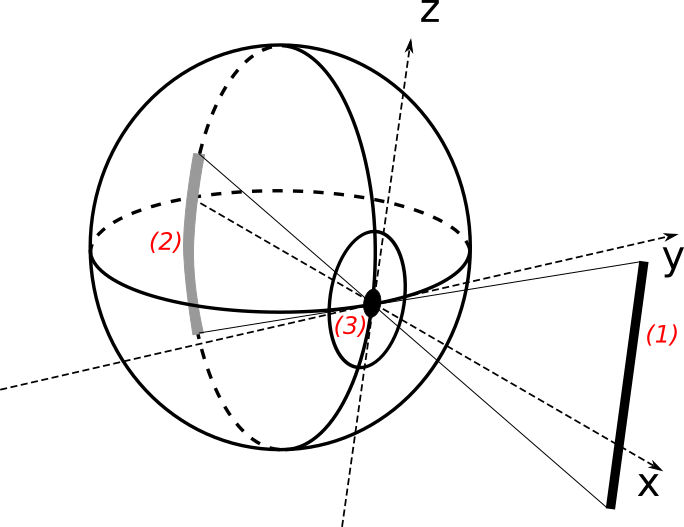
\includegraphics[scale=0.5]{Olho-Tridimensional}
		\caption{Representação Esquemática do Olho Tridimensional.}
		\label{fig:Olho3D}
	\end{figure}

	\paragraph{}
	Na Figura ~\ref{fig:Olho3D}, acima, é possível ver um  \textbf{Objeto (1)} no espaço (posicionado de forma concorrente ao eixo \textbf{x}, na figura), com a sua imagem refletida na \textbf{Retina (2)}. Os raios de luz do objeto passam pela abertura da \textbf{Pupila (3)} e, quanto maior essa abertura, menor a definição da imagem registrada na \textbf{Retina}, mas quanto menor a abertura, maior a definição, mas menos a disponibilidade de luz para formar a imagem.
	
	\paragraph{}
	A principal característica do olho tridimensional é a sua retina bidimensional, e toda a realidade e todas as imagens obtidas a partir do espaço 3D, na verdade, são projeções sobre uma superfície.
	
	\begin{figure}[h]
		\centering
		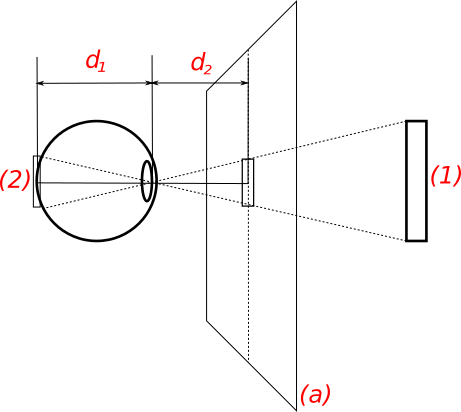
\includegraphics[scale=0.7]{Desenvelope-Da-Retina}
		\caption{Desenvelopando a Projeção Estereográfica do Espaço, na Retina, para um Plano.}
		\label{fig:DesenvelopeRetina3D}
	\end{figure}
	
	\paragraph{}
	Como toda a realidade tridimensional é mapeada em uma superfície bidimensional, podemos dizer que o que o olho percebe é uma projeção estereográfica de metade do espaço tridimensional. O que está atrás do olho não pode ser mapeado, somente o que está à frente. Na Figura ~\ref{fig:DesenvelopeRetina3D}, acima, vemos a \textbf{Imagem (2)} do \textbf{objeto (1)} projetado na Retina e, então, desenvelopado em uma \textbf{superfície plana (a)}. A retina tem uma certa profundidade $\boldsymbol{d_1}$ e a sua imagem pode ser desenvelopada em qualquer superfície a qualquer distância $\boldsymbol{d_2}$. Se fizermos ao contrário, projetando a realidade (ou alguma imagem representando alguma realidade) na superfície \textbf{(a)}, e posicionarmos tal projeção perante o olho, este será enganado e perceberá tal projeção como a própria realidade. Esse é o princípio de funcionamento das televisões, computadores e cinema.
	
	\paragraph{}
	Essa é apenas uma apresentação básica do Olho Tridimensional e não vamos entrar em mais detalhes a respeito de seu modelamento, porque esse já é um problema bem resolvido, sendo até mesmo assunto de Ensino Médio. Mas podemos usar esse modelo de olho 3D para apresentarmos o modelo de olho 2D para visualizar a realidade tridimensional.
	 
	\subsection{Modelo de Olho 2D} \label{mo2d}
	
	\paragraph{}
	O olho 2D, diferentemente do olho 3D, existe apenas em um plano. Mas, no caso desse estudo, esse plano está contido em um espaço tridimensional. Uma representação visual desse olho pode ser vista na Figura ~\ref{fig:Olho2D}, abaixo. Deve-se esclarecer que, na figura do Olho Bidimensional, ele está posicionado no plano \textbf{xy}, sendo o eixo \textbf{z} ortogonal a esse "olho". Podemos ver nessa figura a \textbf{Retina (2)} e a \textbf{Pupila (3)}. Ambas unidimensionais. Vemos que o objeto é colapsado para uma curta linha, no centro da retina linear.
	
	\paragraph{}
	Segundo o senso comum, assume-se que um olho bidimensional como esse não tem condições de perceber toda a realidade tridimensional e, se o fizer, a perda de informação é muito grande para tal visualização fazer sentido. Entretanto, mesmo a capacidade visual que temos com os nossos olhos tridimensionais permitem apenas a percepção de uma projeção, com enorme perda de informação, que é contrabalanceada pela nossa capacidade de navegarmos por dentro do espaço 3D.
	
	\begin{figure}[h]
		\centering
		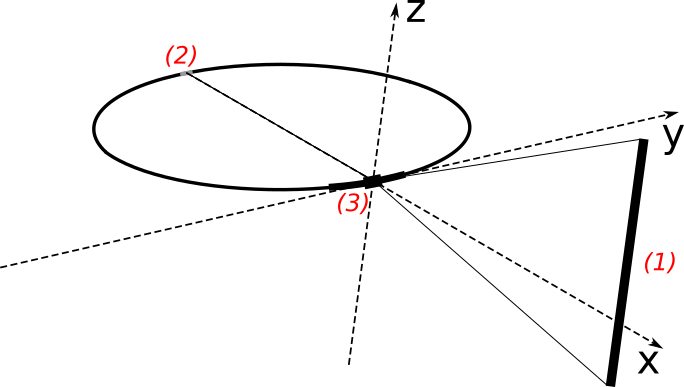
\includegraphics[scale=0.7]{Olho-Bidimensional}
		\caption{Representação Esquemática de um Olho Bidimensional Flutuando no Espaço 3D.}
		\label{fig:Olho2D}
	\end{figure}
	
	\paragraph{}
	Assim, podemos considerar critérios de representação do espaço tridimensional em um olho bidimensional, com uma retina unidimensional e, dados critérios que reduzam ao máximo a perda de informação, podemos adicionar critérios de navegação (movimentação) desse olho no espaço tridimensional, de forma a recuperar a informação faltante.
	
	\subsection{Critérios de Visualização e Interação 3D para 2D} \label{criterios}
	
	\paragraph{}
	Agora que temos um modelo de olho bidimensional que pode enxergar tridimensionalmente, podemos formalizar a forma que a luz chega na retina bidimensional para criar uma imagem unidimensional representando a realidade tridimensional.
	
	\paragraph{}
	Uma característica marcante desse olho 2D mergulhado no espaço 3D é que os raios de luz que chegam a esse olho provêm de todo o espaço, não apenas do Plano \textbf{xy}, onde tal olho reside. Quando os raios de luz não chegam a partir do Plano \textbf{xy}, ele possui um componente perpendicular ao olho. Esse componente é perdido, mas o olho ainda pode ver a projeção no Plano \textbf{xy} de tal vetor de luz. Obviamente, para representar essa captura de raio de luz não diretamente direcionado à retina, precisamos definir uma perda, e essa perda é justamente o componente em \textbf{z} desse raio de luz. Como todos os raios de luz que possuam uma componente \textbf{z} qualquer mas as mesmas componentes \textbf{x} e \textbf{y} vão ser representados no mesmo ponto na retina bidimensional, podemos dizer que tal olho bidimensional possui uma \textbf{"reta de vista"}, não um ponto de vista - e podemos combinar todos os pontos dessa reta, considerando a perda do componente z e o uso da técnica de \textit{alpha-blending} (também chamado de \textit{alpha compositing}, mas em um contexto completamente diverso - daí preferirmos o termos \textit{blending}) (\citep[p.~56]{2015MajiNath}). Utilizando os principios de \textit{ray-tracing} e de \textit{radiosity} (\citep[]{1995CoWall}), podemos combinar esses pontos da reta de vista de uma forma racional. Esse é o \textbf{Critério da Direção}.
	
	\paragraph{}
	Todos os pontos da realidade, se eles representam fontes de luz, possuem uma perda de luminosidade (\cite{2012Bukshtab}) até chegar a retina do olho bidimensional. Essa perda permite reduzir a representação de objetos a grandes distâncias, para dar mais importância à representação dos objetos mais próximos e relevantes. Além disso, se um objeto mais distante tiver seu raio de luz interceptado por um objeto mais próximo, passa a valer o raio de luz do objeto mais próximo. Esse é o \textbf{Critério da Distância}.
	
	\paragraph{}
	A retina do olho bidimensional funciona de forma similar à retina tridimensional e quanto maior a sua abertura, menor a qualidade da imagem formada. Entretanto, um detalhe da abertura do olho que não pode passar despercebido é que o angulo sólido que o olho capta para a formação da imagem cobre uma superfície limidada da abóboda da retina e o olho percebe um parte limitada do firmamento (\cite{2018Diaz}). Isso também tem a ver com a abertura da pupila e com a sensitividade das regiões da retina, havendo, inclusive um ponto específico de maior sensitividade, a \textbf{fóvea}(\cite{2022Rehman}). O controle da abertura da área de captura de luz e da pupila define o \textbf{Critério da Abertura}.
	
	\paragraph{}
	Os critérios acima são utilizados para representar a realidade 3D como uma imagem 2D, ou, no caso do Olho Bidimensional, como uma imagem 1D. Essa imagem formada possui grande perda de informação. Então, para recuperar a informação perdida, precisamos movimentar o foco do olho para diversas direções, de forma a capturarmos o máximo de informações do ambiente e, então, reconstruir mentalmente o espaço. Podemos andar em três eixos e girar em três eixos - ou seja, estaremos trabalhando com seis graus de liberdade. E, movimentando-nos, utilizando da nossa capacidade de paralaxe, podemos trabalhar para construir a realidade como um todo. Esse é o \textbf{Critério da Navegação}. \footnote{Um elemento relevante do Critério da Navegação é a utilização de \textbf{dois} olhos para a formação da imagem mental com sentido de profundidade. Esse elemento é tão relevante que poderia ser definido como um critério à parte (o \textbf{Critério da Estereoscopia}, sendo este um critério interacional). Mas ele é absurdamente complexo de se modelar e, para o projeto que estamos fazendo, tanto para a redução de $\R^3 \Rightarrow \R^1$ quanto para a redução de $\R^4 \Rightarrow \R^2$, \textbf{completamente secundário}. Desenvolver um simulador quadridimensional estereoscópico está fora do escopo desse trabalho e dos trabalhos seguintes, podendo ser uma extensão a ser desenvolvida no longuíssimo prazo - assim como o desenvolvimento do projeto em Realidade Aumentada ou Realidade Virtual. O Critério da Navegação parece ser uma inovação apresentada por esse projeto. Ainda estou procurando por referências adequadas.}
	
	\paragraph{}
	Não vamos entrar em detalhes matemáticos de cada um dos critérios, pois explorá-los, formalizá-los e utilizá-los como modelo para a generalização desse método para perceber um espaço quadridimensional em um olho tridimensional é a proposta final dessa pesquisa. A implementação das coordenadas do olho 2D no Espaço 3D e sua navegação, reposicionando todos os pontos do espaço é uma aplicação da movimentação de um \textbf{Referencial de Frenet} no espaço 3D, levando a crer que essa pesquisa tenha que tratar de elementos de \textbf{Geometria Diferencial}. E a representação dos objetos 3D na projeção 1D parece ser uma aplicação de \textbf{Geometria Computacional}, que depende fortemente de conhecimentos de \textbf{Geometria Analítica}, \textbf{Cálculo Vetorial} e \textbf{Álgebra Linear}.
	
	\paragraph{}
	Uma vez modelado o olho bidimensional, devemos fazer o desenvelope da retina mapeada e criar uma projeção animada 1D da realidade 3D para que voluntários testem esse modelo de olho bidimensional. 
		
	\section{Implementação - Ferramentas de Desenvolvimento Propostas} \label{if}
	
	\paragraph{}
	Essa proposta de pesquisa envolve o desenvolvimento de software para que pessoas, voluntários, interajam com ele e seja possível avaliar a sua capacidade de interagir com um espaço tridimensional, apenas visualizando esse espaço em uma projeção unidimensional.
	
	\paragraph{}
	As ferramentas de software tradicionais em Computação Científica (\textbf{R}\footnote{\url{https://www.r-project.org/}}, \textbf{Python}\footnote{\url{https://www.python.org/}} e \textbf{Julia}\footnote{\url{https://julialang.org/}}) têm como característica comum o péssimo suporte a compilação e empacotamento de executáveis para distribuição. Assim, declinamos do uso delas para a geração do software necessário a ser distribuído a terceiros, para testar as hipóteses levantadas nessa proposta de projeto. As linguagens e compiladores com excelente suporte a distribuição de software, e fortemente utilizadas na academia são \textbf{Fortran}\footnote{\url{https://fortran-lang.org/en/}}, \textbf{C}\footnote{\url{https://www.iso.org/standard/74528.html}} e \textbf{C++}\footnote{\url{https://isocpp.org/}}. Assim, uma dessas três linguagens/compiladores poderia ser escolhida/escolhido para o desenvolvimento desse projeto.
	
	\paragraph{}
	O projeto aqui apresentado vai lidar com grande volumes de informações, para ser possível a representação de um espaço tridimensional. Para processar esse volume imenso de pontos, é necessário o suporte adequado de Hardware. Para tanto, o cálculo em nível vetorial necessitará ser feito com auxílio de placas de processamento 3D. A interface com essas placas pode ser feita através das APIs (de \textit{Application Program Interface}) tradicionais de Cálculo Vetorial, como \textbf{OpenGL}\footnote{\url{https://www.opengl.org/}}, \textbf{Vulkan}\footnote{Também embaixo do padrão \textbf{OpenGL}} ou \textbf{Direct3D}\footnote{Direct3D é uma tecnologia proprietária da Microsoft, e só é adequada a ser executada em Windows\texttrademark: \url{https://learn.microsoft.com/en-us/windows/win32/direct3d}}, ou mesmo APIs mais modernas de Cálculo Numérico, como o \textbf{Cuda}\footnote{\url{https://developer.nvidia.com/cuda-zone}}.
	
	\paragraph{}
	Entretanto, o software desenvolvido nesse projeto é para ser distribuído a terceiros e quanto mais fácil essa distribuição, melhor para a coleta de dados e para a avaliação da pesquisa. Para tanto, foi escolhida a distribuição Web - ou seja, desenvolver o sistema de forma que ele possa ser carregado dentro de um Website. Assim, cria-se um Website público e é necessário apenas compartilhar o seu endereço com os voluntários, para que a pesquisa de campo seja feita. Das APIs de Cálculo Vetorial, com aceleração de hardware, a única disponível para Web é a \textbf{OpenGL}, através da biblioteca \textbf{Emscripten}\footnote{\textbf{\url{https://github.com/emscripten-core/emscripten}}}, que permite compilar \textbf{C} e \textbf{C++} para web. Como \textbf{Fortran} não é suportado pela \textbf{Emscripten}, tal linguagem foi desconsiderada para o \textit{toolchain}.
	
	\paragraph{}
	Considerando todas as restrições acima, apenas \textbf{C} e \textbf{C++} são elegíveis para o desenvolvimento do projeto. Obviamente, elementos decorativos e subsidiários, como layout da página que vai hospedar o projeto e a interatividade inicial básica, devem ser desenvolvidos utilizando-se \textbf{HTML}\footnote{\url{https://html.spec.whatwg.org/}}, \textbf{CSS}\footnote{\url{https://www.w3.org/TR/CSS/\#css}} e \textbf{Javascript}\footnote{\url{https://www.ecma-international.org/publications-and-standards/standards/ecma-262/}}. Mas essa parte de código do projeto deve se manter mínima e sem representar nenhum interesse acadêmico. Por conta da disponibilidade de bibliotecas com suporte a diversos algoritmos de computação científica, disponíveis nos \textbf{Emscripten Ports}\footnote{\url{https://github.com/emscripten-ports}}, para \textbf{C++}, como o \textbf{Boost}\footnote{\textbf{\url{https://www.boost.org/}}}, além de sua excelente biblioteca de estruturas de dados, a \textbf{STL}\footnote{A \textbf{STL} é a \textit{Standard Template Library} é, e faz parte da Biblioteca Padrão da linguagem \textbf{C++}}, foi escolhida a linguagem \textbf{C++} para esse projeto.
	
	\paragraph{}
	Todas as ferramentas acima são para o desenvolvimento do software que os voluntários irão interagir. Entretanto é necessário ter um software específico para recolher os dados das interações dos usuários e armazená-los, para análise ulterior. Para tanto, um servidor é necessário, com um banco de dados para receber as informações. O servidor pode ser hospedado no Sistema Operacional \textbf{Linux}\textregistered, distribuição \textbf{Ubuntu}\texttrademark\footnote{\url{https://ubuntu.com/}}, com banco de dados relacional \textbf{PostgreSQL}\footnote{\url{https://www.postgresql.org/}}, e uma camada \textit{backend} feita na Linguagem de Programação \textbf{Go}\footnote{\url{https://go.dev/}}, porque ela permite o desenvolvimento de \textit{backends} muito enxutos e, portanto, muito baratos de se hospedar. \textit{Obs.:} Pensou-se em utilizar um banco de dados não relacional (como o \textbf{MongoDB}\footnote{\url{https://www.mongodb.com/}}), mas esses bancos de dados não relacionais não são utilizados largamente para pesquisa acadêmica, sendo, então, desconsiderados, enquanto bancos de dados relacionais são largamente suportados academicamente, incluindo até uma algebra própria deles.
	
	\paragraph{}
	A hospedagem web e o endereço DNS público para hospedar o sistema será fornecido pelo autor desse projeto.
	
	\paragraph{}
	Assim o \textit{toolkit} escolhido para o desenvolvimento dessa proposta de pesquisa foi:
	
	\begin{itemize}
			\item Plataforma de Distribuição: Web (Página distribuída na Internet, sob protocolo HTTP e acessível no navegador)
			\item Linguagens de Programação: \textbf{C++}, para o projeto principal, \textbf{Javascript}, \textbf{CSS} e 	\textbf{HTML} para as páginas de suporte \textit{frontend} para levar os voluntários ao projeto e a linguagem \textbf{Go} para o suporte \textit{backend}.
			\item Ferramenta de Compilação, Construção e Empacotamento: \textbf{Emscripten}
			\item Bibliotecas de Suporte principais: \textbf{Boost}, \textbf{OpenGL}, \textbf{C++ STL}
			\item Biblioteca de Cálculo Vetorial: \textbf{OpenGL}, através da biblioteca \textbf{GLM}		
			\item Hospedagem do Projeto sobre sistema operacional \textbf{Linux}, distribuição \textbf{Ubuntu}.	
			\item Banco de Dados relacional \textbf{PostgreSQL}.
	\end{itemize}
	
	\section{Implementação - Entregáveis Propostos} \label{ie}
	\paragraph{}
	Os entregáveis propostos para essa pesquisa são:
	
	\begin{itemize}
		\item A própria estrutura do Website para hospedar o projeto. A hospedagem em si está fora do escopo dessa proposta.
		\item O componente de software, em \textbf{WASM}\footnote{\url{https://webassembly.org/}} com o sistema que representa uma realidade 3D simulada, visível apenas através de uma retina 2D.
		\item O conjunto de dados das interações dos voluntários, capturados e disponibilizados para análise.
		\item A análise desses conjuntos de dados.
		\item O relatório com toda a metodologia de análise e as conclusões tiradas.
		\item Uma proposta de extensão dessa pesquisa para a representação de uma simulação 4D a ser visualizada através de uma retina 2D, como as que os seres humanos possuem no nosso universo real.
	\end{itemize}
	
	\section{Pesquisa de Campo - Interação Pública} \label{pc}
	\paragraph{}
	A pesquisa de campo para esse projeto é feita através do uso do software distribuído pela internet por voluntários, que podem ou não ser anônimos.
	
	\paragraph{}
	Como os voluntários interagirão com um software, toda a coleta de dados pode ser automatizada, e um conjunto de interações previsíveis e objetivas pode ser definida para os voluntários seguirem, de forma que o software disponibilizado será muito parecido com um jogo eletrônico.
	
	\paragraph{}
	Não será descrita nessa proposta que conjunto de interações serão essas definidas para os usuários cumprirem, mas elas deverão ser cuidadosamente preparadas e roteirizadas para que se avalie se as pessoas conseguem navegar e interagir adequadamente em um ambiente tridimensional tendo acesso a apenas um mecanismo de visão unidimensional. A interação pode ser feito pelo Teclado do Computador ou através de \textit{joysticks}, e ambas formas de interação devem ser cuidadosamente preparadas, considerando os aspectos ergonômicos que surgirem.
	
	\paragraph{}
	Não está claro ainda, nessa proposta, como definir grupos de controle e qual é o volume de pessoas que é necessário para uma amostra estatísticamente relevante. Ajuda de especialistas em \textbf{Percepção e Interatividade}, ou mesmo \textbf{Neurociência}, ou \textbf{Psicologia e Comportamento}, será necessária para definir os roteiros de interação. Como o projeto será distribuído pela Internet, então é possível, dado o trabalho adequado de divulgação, atingir um conjunto de voluntários na casa de milhares de pessoas: ou seja, esse projeto pode, inclusive, considerar elementos de \textbf{Estatística} mais sofisticados do que uma inferência básica.

	\section{Conclusão} \label{c}
	
	\paragraph{}
	Partindo de uma premissa bastante simples, a possibilidade de um ser bidimensional perceber a realidade tridimensional, chegou-se a uma proposta de Iniciação Científica bastante profunda, com grande nível de interdisciplinaridade.
	
	\paragraph{}
	Se a tese da capacidade humana de perceber a realidade tridimensional apenas visualizando uma realidade bidimensional for comprovada (o que parece ser bastante plausível, uma vez que cegos lidam com a realidade tridimensional sem enxergar), parte-se para a próxima etapa dessa pesquisa: avaliar a capacidade humana de perceber o espaço quadridimensional, e mesmo desenvolver intuições quadridimensionais, quando vivemos em uma realidade espacial tridimensional.
	
	\paragraph{}
	Nesse caso de perceber o espaço 4D, a única opção que temos é através da simulação, porque não é possível ter um espaço quadridimensional disponível para testarmos as nossas limitações de percepção. Esse espaço 4D simulado deverá ser navegado e interagido de forma mediada. Uma preparação cuidadosa de interfaces através do teclado do computador e de \textit{joysticks} deve ser desenvolvida, e essa interface deve funcionar como uma \textbf{extensão maquínica} que leva as pessoas para dentro do espaço quadridimensional. Uma das hipóteses é a capacidade de \textbf{cognição incorporada}(\cite{2021Shapiro}) (do inglês \textit{embodiment}/\textit{embodied cognition}) das pessoas permitirem que elas sejam transportadas virtualmente para o espaço quadridimensional e consigam interagir com esse espaço com sucesso e, então, desenvolver intuições e \textit{insights} quadridimensionais.
	
	\paragraph{}
	A estrutura de projeto para a percepção do espaço 4D é exatamente a mesma estrutura desse projeto e, provavelmente, as bases teóricas em Matemática e nas outras ciências são exatamente as mesmas, também. Assim, os três critérios de representação, o \textbf{Critério da Direção}, o \textbf{Critério da Distância} e o \textbf{Critério da Abertura}, e o critério de interação, o \textbf{Critério da Navegação}, podem ser devidamente estendidos para o modelamento de espaços 4D (ou mesmo de dimensões ainda superiores) visualizáveis e interativos a seres tridimensionais. 
	
	\paragraph{}
	De toda forma, fica a expectativa de, primeiro, se construir o projeto de visualização e percepção 3D em 1D, para, depois, partir para a percepção 4D por seres do espaço 3D. Mesmo o uso de realidade virtual pode ser possível para esses experimentos.
		
	\bibliographystyle{plainnat}
	\bibliography{3D1D-Bibliography.bib}
\end{document}